% ********** Rozdział 3 **********
\newpage
\chapter{Harmonogram realizacji projektu}

W niniejszym rozdziale przedstawiono harmonogram realizacji projektu w formie diagramu Gantta. Diagram ten ilustruje poszczególne etapy projektu oraz ich czas trwania.

\begin{figure}[h]
    \centering
    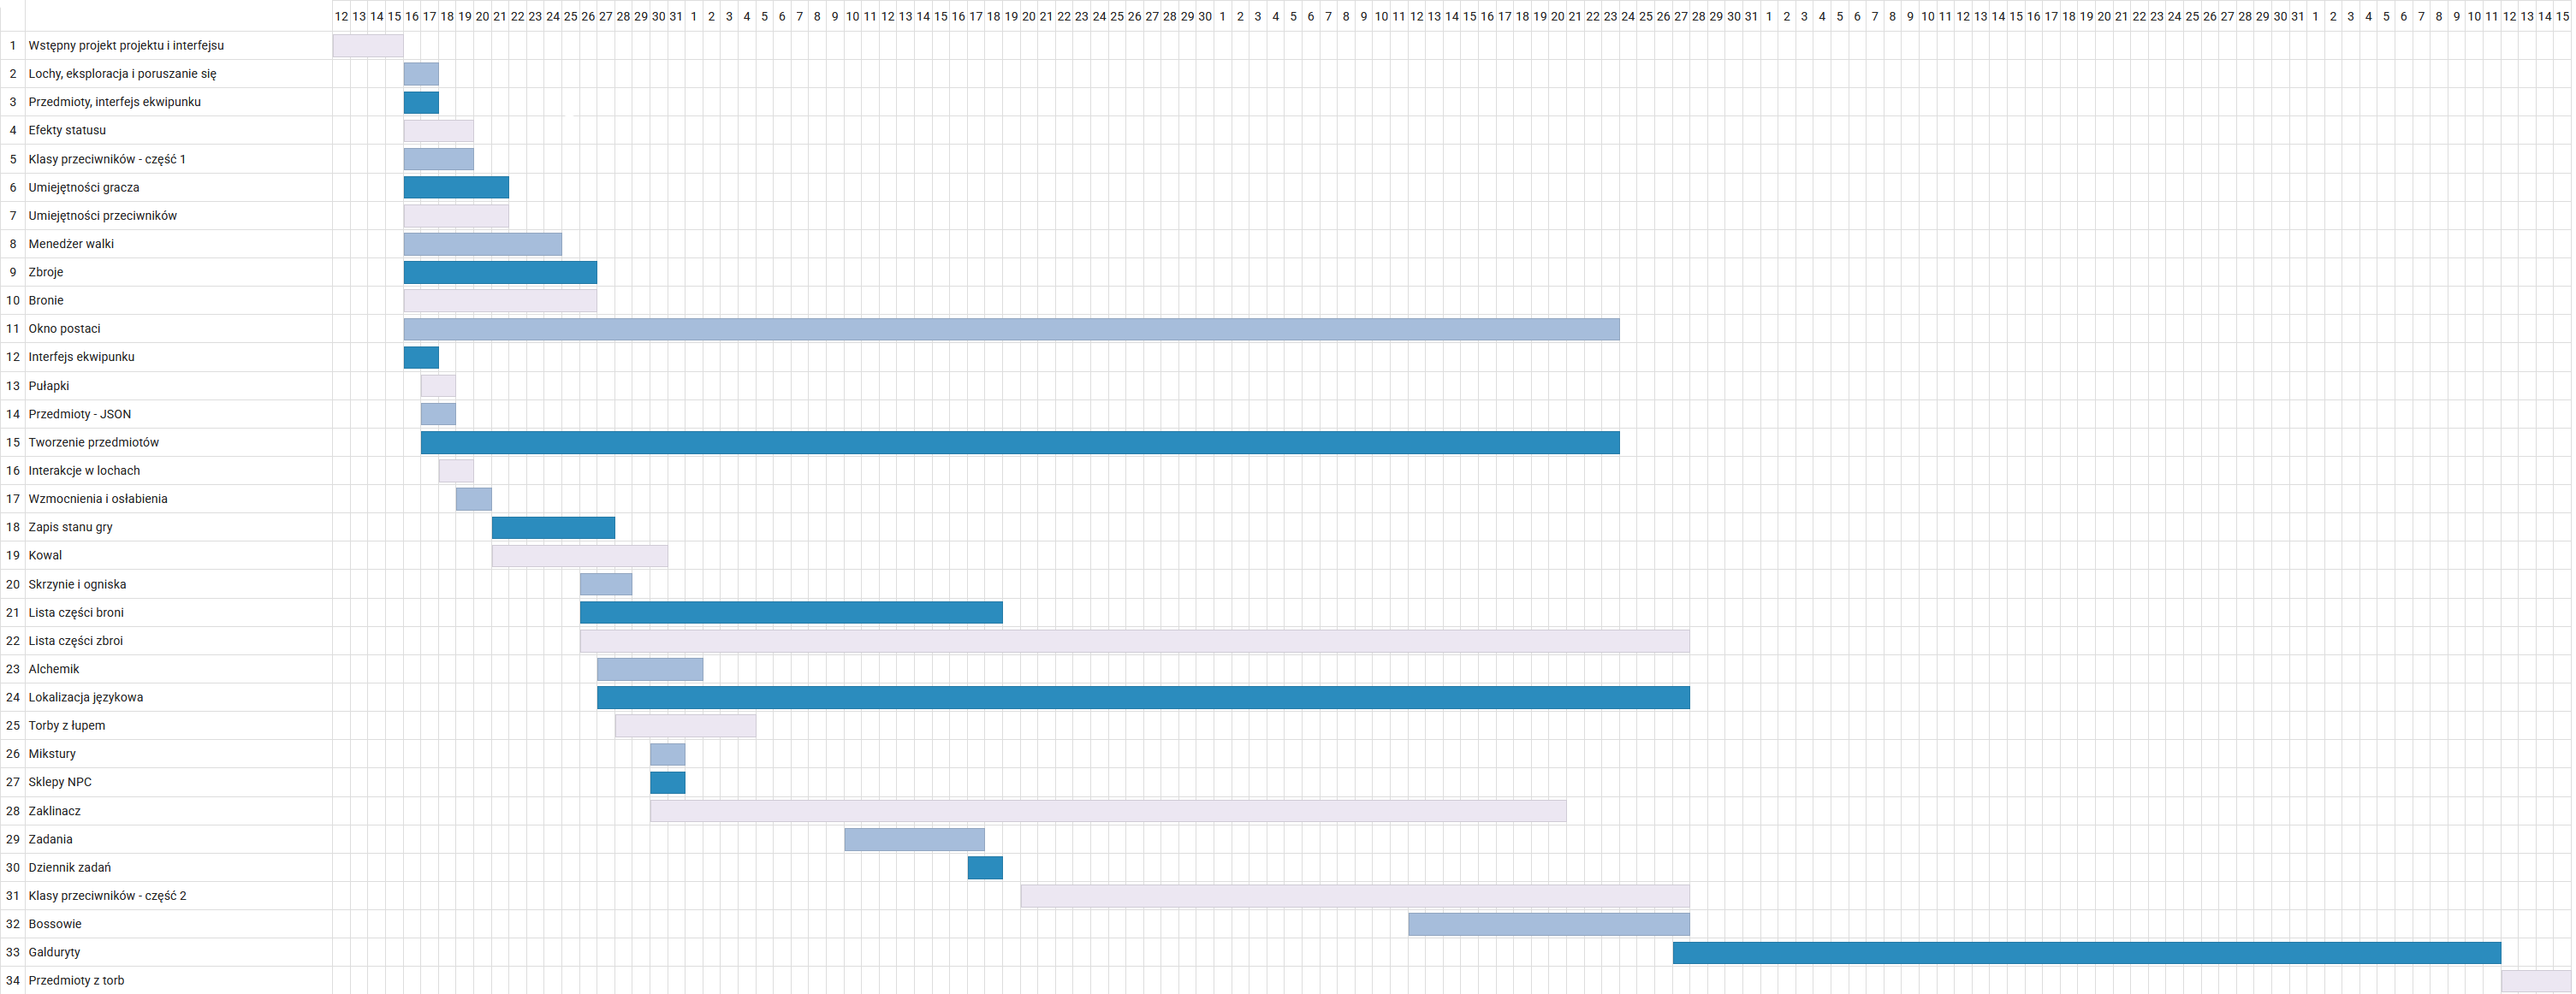
\includegraphics[width=\textwidth]{figures/gantt.png}
    \caption{Diagram Gantta przedstawiający harmonogram realizacji projektu.}
    \label{fig:gantt_chart}
\end{figure}

\section{Problemy i trudności}
Podczas realizacji projektu napotkano kilka trudności, w tym:
\begin{itemize}
    \item \textbf{Niedoszacowanie czasu} - Wstępne oszacowania czasowe okazały się niewystarczające, co prowadziło do opóźnień.
    \item \textbf{Konieczność refaktoryzacji} - Niedopracowanie niektórych struktur projektu wymagało przeplanowania i dokonania refaktoryzacji, co również opóźniło ukończenie projektu
    \item \textbf{Problemy z integracją} - Integracja różnych komponentów systemu (np. JSON) napotkała na nieprzewidziane trudności techniczne.
\end{itemize}

\section{Repozytorium i system kontroli wersji}
Projekt jest zarządzany w systemie kontroli wersji Git, a wszystkie zmiany są dokumentowane w repozytorium dostępnym pod adresem: \url{https://github.com/xzantem/ConsoleGodmist}. 
Użycie systemu kontroli wersji umożliwiło śledzenie postępów, kontrolę wprowadzanych zmian i łatwe cofanie do poprzednich wersji.


% ********** Koniec rozdziału **********
